\documentclass[french]{article}

% Language setting
% Replace `english' with e.g. `spanish' to change the document language
\usepackage[french]{babel}

% Set page size and margins
% Replace `letterpaper' with`a4paper' for UK/EU standard size
\usepackage[a4paper,top=2cm,bottom=2cm,left=3cm,right=3cm,marginparwidth=1.75cm]{geometry}

% Useful packages
\usepackage{amsmath}
\usepackage{graphicx}
\usepackage[colorlinks=true, allcolors=blue]{hyperref}
\usepackage{listings}
\usepackage[utf8]{inputenc}
\usepackage[T1]{fontenc}
\pagestyle{empty} %% très important !


\title{Application de l'analyse de classification aux accidents de la circulation routière en France}
\author{Juan Diego Alfonso, Laure Gentili , Tiavina Andriamisaina, Marwan Ait Addi}
\date{Novembre 2023}

\begin{document}
\maketitle

\begin{abstract}
Depuis la popularisation de l'automobile, les chercheurs étudient les accidents de la route dans le but d'améliorer la sécurité des usagers. \cite{rapport-accident-canada}. Dans cette étude, nous cherchons à utiliser des techniques modernes de science des données pour classifier les accidents de la route en France, afin d’identifier les facteurs de risque associés. Pour ce faire, nous utilisons des données provenant de \href{http://data.gouv.fr/}{data.gouv.fr}, que nous analysons à l'aide d’un algorithme de forêt aléatoire. Les résultats de cette étude nous permettrons de déterminer les facteurs qui influent la gravité d’un accident et de proposer des moyens pour les éviter.
\end{abstract}

\tableofcontents 

\section{Introduction}
En 2022, l’Observatoire national interministériel a enregistré 3 267 décès liés à des accidents de la route en France métropolitaine, soit une hausse de 11\% par rapport à l’année 2021. La sécurité routière est un enjeu majeur dans la société actuelle, ayant des répercussions directes sur la vie des individus.

Malgré les efforts déployés en terme d’infrastructures et de sensibilisation, le nombre de décès et de blessés sur les routes françaises reste trop significatif. Il est important de comprendre et d’identifier les facteurs déterminants afin de concevoir des stratégies toujours plus efficaces pour réduire le nombre de victimes. 

Afin de saisir et de prévenir les facteurs menant à ces accidents, l’adoption d’une approche moderne et automatique s’avère nécessaire. Dans cette optique, cet article se focalise sur l’utilisation d’un outil d’apprentissage automatique, le RandomForestClassifier, dans le but de classifier les accidents routiers en France. Bien que de nombreux articles ont déjà traités la question des accidents routiers en France, la plupart n’ont utilisé que des approches limités, telles que des statistiques descriptives, qui ne sont pas suffisamment efficaces pour explorer en profondeur la complexité de ce sujet.

\section{État de l'art}
Les études évaluées dans divers articles ont permis d’identifier l’évolution de la collecte de données sur les accidents de la route. Cette collecte s'est grandement améliorée au fil du temps, visant à accroître sa précision. L’objectif était d’enrichir les modèles existants et de mieux identifier les inconvénients et les avantages des éléments trouvés. Ces données ont également été soumises à des comparaisons avec celles obtenues par d’autres méthodes de collecte.

L’étude présentée dans cet article se repose sur les données collectées et publiées par le gouvernement français, accessibles sur \href{http://data.gouv.fr/}{data.gouv.fr}. Ces informations offrent une compilation détaillée des données recueillies de 2008 à 2022.

En tenant compte d’autres articles scientifiques, nous avons pu identifier les valeurs nécessaires à prendre en considération dans nos études précédentes, le type d’informations recueillies, et comment les traiter de manière plus efficace, en les classant selon les méthodes choisies dans cet article.

A partir des années 70, les chercheurs s’intéressent déjà aux accidents routiers en France. 
\begin{itemize}
    \item En 1970, J.L’Hoste \cite{etude-clinique-accidents} dresse une première analyse du recueil des données prises par les forces de l’ordre. Il examine la méthodologie des américains Baker, J-S et al de 1960 afin de proposer une amélioration dans la collecte d’informations et l’analyse des accidents de la route.
    \item En mai 1964, le ministère des transports du Québec \cite{rapport-accident-canada} publie un dossier d’analyse et de classification des accidents de la route. Ainsi, nous pouvons accéder au formulaire de rapport d’accident utilisé par les forces de l’ordre et nous permet de mieux comprendre comment les accidents sont notés et enregistrés dans des bases de données pour être ensuite analysées.
    \item En 1975, J.Vallin et J-C.Chesnais \cite{accidents1953} examinent les données depuis 1953, se concentrant sur l’évolution de la mortalité routière en France, en utilisant des statistiques descriptives. Ils concluent à une insuffisance dans les moyens mis en place pour lutter contre les accidents de la route. Bien que précurseure, cette analyse est bien trop légère et ne permet pas de comprendre en profondeur comment lutter contre ces accidents.
    \item En 2003, Hélène Fontaine \cite{FONTAINE2003107} établit un premier lien entre la gravité d’un accident routier et l’âge du conducteur. En se penchant sur les caractéristiques des conducteurs âgés et la proportion des accidents impliquant ces derniers, elle conclut que la gravité d’un accident augmente avec l’âge du conducteur. Bien qu’elle ne se penche que sur une variable, son analyse très complète permet d’identifier avec précision un premier facteur déterminant dans les accidents de la route.
    \item En 2011, S.Shanti et Dr.R.Geetah Ramani \cite{classification-colision} étudient la classification des collisions de véhicules en utilisant des algorithmes de Data Mining. Leur analyse très complète compare plusieurs algorithmes, démontrant l’efficacité de l’algorithme Random Tree pour classifier les accidents. Ainsi, cette étude constitue le pilier de notre analyse.
\end{itemize}

\section{Dataset}
Les données exploitées proviennent du ministère de l'Intérieur et répertorient tous les accidents corporels de la circulation enregistrés par les forces de l'ordre. Initialement, ces données étaient organisées en quatre tableaux distincts, chacun détaillant différentes caractéristiques des accidents :
\begin{itemize}
    \item \textbf{Caractéristiques} : Ce tableau offre une description des circonstances générales entourant chaque accident.
    \item \textbf{Lieux} : Ce tableau fournit des informations sur l'emplacement précis de chaque accident.
    \item \textbf{Véhicules} : Ce tableau présente des détails sur le ou les véhicules impliqués dans chaque incident.
    \item \textbf{Usagers} : Ce tableau offre des informations sur les personnes impliquées dans chaque accident.
\end{itemize}

Par la suite, nous avons consolidé ces données dans un unique tableau afin de faciliter le processus de nettoyage. Le jeu de données utilisée regroupent ainsi 126 658 accidents répertoriés. En annexe, vous trouverez une liste des exhaustive des caractéristiques que nous avons retenues pour notre analyse.

\subsection{Nettoyage, collecte et pré-traitement des données}
Lors de l’évaluation initiale de nos données, nous avons constaté qu’elles bénéficiaient déjà d'une structuration et d'une normalisation efficace grâce à un pré-nettoyage préalable effectué par la source des données. Ce pré-nettoyage a grandement simplifié notre processus ultérieur. Les données, provenant d’une source fiable, étaient organisées en tableaux facilement identifiables et ne présentaient pas d’irrégularités majeures.

Néanmoins, quelques ajustements ont été nécessaires pour adapter les données à notre méthodologie d’étude. Certains formats ne correspondaient pas avec notre approche d’analyse, nécessitant ainsi des modifications appropriées. De plus, nous avons repéré quelques valeurs supplémentaires non pertinentes pour notre étude.

La nécessité de nettoyer des caractères spéciaux ou d’éliminer les valeurs nulles ne s'est pas présentée, car ces problèmes étaient absents de notre ensemble de données. Les valeurs aberrantes identifiées ont été gérées efficacement grâce à l’encodage à chaud (one hot encoding).

Notre objectif principal lors du nettoyage des données était de parvenir à extraire les informations les plus pertinentes pour notre étude. Nous avons accordé une priorité particulière aux éléments clés, visant à rendre les variables de notre modèle aussi précises que possible. Cette approche nous a permis d’identifier des valeurs entre les ensembles de données qui méritaient d'être éliminées ou incluses dans nos résultats finaux.

En somme, bien que nos données étaient initialement bien traitées, nous avons effectué un nettoyage minutieux pour garantir la précision et la pertinence de notre analyse.

Suite à cette étape, nous avons procédé au pré-traitement des données analytiques présentées dans l’analyse descriptive. Nous avons joint les quatre tables mentionnées précédemment en utilisant la valeur commune \verb|num_acc|, permettant ainsi l’unification de toutes les données d’une seule année en un seul ensemble de données.

\subsection{Statistiques descriptives du dataset}
Avant d’analyser les liens entre les différents facteurs liés aux accidents, il est pertinent d’explorer les données afin de mieux les comprendre et de sélectionner les variables pertinentes. Dans cette perspective, nous avons préalablement effectué une analyse descriptive du jeu de données.
\begin{table}[h]
\centering
\begin{tabular}{|c|c|c|}
\hline
\textbf{Catégorie usager} & \textbf{Fréquence} & \textbf{Pourcentage} \\
\hline
Conducteur & 94418 & 74.55\% \\
Passager & 22675 & 17.90\% \\
Piéton & 9565 & 7.55\% \\
\hline
\end{tabular}
\caption{Répartition des catégories d'usagers}
\end{table}

\begin{table}[h]
\centering
\begin{tabular}{|c|c|c|}
\hline
\textbf{Tranche d'âge} & \textbf{Fréquence} & \textbf{Pourcentage} \\
\hline
1920-1940 & 2377 & 1.88\% \\
1940-1960 & 13111 & 10.35\% \\
1960-1980 & 31507 & 24.88\% \\
1980-2000 & 48515 & 38.30\% \\
2000 et après & 28270 & 22.32\% \\
Non renseigné & 2878 & 2.27\% \\
\hline
\end{tabular}
\caption{Répartition des tranches d'âge}
\end{table}
\begin{table}[h]
\centering
\begin{tabular}{|p{6cm}|c|c|}
\hline
\textbf{Type de collision} & \textbf{Fréquence} & \textbf{Pourcentage} \\
\hline
Deux véhicules - frontale & 15053 & 11.88\% \\
Deux véhicules – par l’arrière & 18481 & 14.59\% \\
Deux véhicules – par le côté & 39844 & 31.46\% \\
Trois véhicules et plus – en chaîne & 8368 & 6.61\% \\
Trois véhicules et plus - collisions multiples & 6545 & 5.17\% \\
Autre collision & 30310 & 23.93\% \\
Sans collision & 7931 & 6.26\% \\
Non renseigné & 126 & 0.10\% \\
\hline
\end{tabular}
\caption{Répartition des types de collisions}
\end{table}

\begin{table}[h]
\centering
\begin{tabular}{|c|c|c|}
\hline
\textbf{Genre} & \textbf{Fréquence} & \textbf{Pourcentage} \\
\hline
Homme & 84793 & 66.95\% \\
Femme & 39121 & 30.89\% \\
Non renseigné & 2744 & 2.17\% \\
\hline
\end{tabular}
\caption{Répartition des genres}
\end{table}

\begin{table}[h]
\centering
\begin{tabular}{|c|c|c|}
\hline
\textbf{Gravité de blessure} & \textbf{Fréquence} & \textbf{Pourcentage} \\
\hline
Indemne & 53628 & 42.34\% \\
Tué & 3550 & 2.80\% \\
Blessé hospitalisé & 19260 & 15.21\% \\
Blessé léger & 49979 & 39.46\% \\
Non renseigné & 241 & 0.19\% \\
\hline
\end{tabular}
\caption{Répartition de la gravité de blessure}
\end{table}

\section{Méthodologie}
\subsection{Choix de l’algorithme de classification} 
Pour sélectionner notre algorithme de classification, nous nous sommes appuyé sur l’étude de S.Shanti et Geetah Ramani \cite{classification-colision}, démontrant que l’algorithme de classification Random Forest est le plus performant pour notre cas d’utilisation.

Étant donné que les approches des articles antérieurs se sont révélées trop superficielles, il est important de sélectionner une méthode plus complexe, complète et adaptée à notre jeu de données. Le RandomForestClassifier, en tant qu’algorithme d’apprentissage automatique, offre l’avantage de pouvoir capturer des schémas complexes au sein des données en identifiant des interactions non linéaires entre les différentes variables. En optant pour cette approche moderne, notre objectif est de dépasser les limites des analyses conventionnelles et de fournir des conclusions plus nuancées sur les causes profondes des accidents routiers en France.

L’algorithme Random Forest a été choisi pour plusieurs raisons :

\begin{itemize}
    \item Robustesse aux données déséquilibrées : Dans les données d’accidents de la route, il est possible que certaines classes (par exemple, les types d’accidents) soient sous-représentées, et Random Forest peut gérer ce déséquilibre.
    \item Gestion des variables catégorielles : Les données d’accidents de la route peuvent comporter de nombreuses variables catégorielles, comme le type de véhicule ou les conditions météorologiques. Random Forest peut traiter ce type de données sans avoir besoin de les transformer.
    \item Importance des caractéristiques : Random Forest fournit une mesure de l’importance des caractéristiques, aidant ainsi à comprendre quels facteurs contribuent le plus aux accidents.
    \item Prévention du surapprentissage : Grâce à l’utilisation de multiples arbres de décision et à l’agrégation de leurs résultats, Random Forest peut éviter le surapprentissage, un problème courant dans les modèles de machine learning.
    \item Flexibilité : Random Forest peut être utilisé pour des tâches de classification et de régression, le rendant flexible pour différents types d’analyses.
\end{itemize}

En implémentant le RandomForestClassifier sur un ensemble de données suffisamment grand, notre objectif est d'identifier les caractéristiques spécifiques des accidents routiers qui sont les plus prédictives de leur gravité et de leurs conséquences.

\subsection{Implémentation, training dataset et Hyperparamètres}
Nous avons opté pour l’implémentation des Random Forest de scikit-learn. Pour ce faire, une adaptation de notre jeu de données a été nécessaire pour utiliser des matrices numpy. Le training set est composé de 70\% de nos exemples, sélectionnés aléatoirement avec la fonction sample de la librairie pandas. Afin de tester notre classifieur, nous utilisons le reste des données. Nous avons choisis de classifier sur la colonne \textbf{grav}, représentant la gravité de l’accident, bien qu'il soit possible de choisir une autre colonne.

Pour déterminer les meilleurs hyperparamètres, nous avons effectué une recherche exhaustive (en brute force) des meilleurs paramètres auprès d’une liste prédéfinie de paramètres possibles.

\section{Résultats}
L'algorithme RandomForestClassifier analyse les données en utilisant la gravité de l'accident comme variable cible. L'objectif est de déterminer si l'algorithme prédit correctement celle-ci afin de comprendre quels facteurs interviennent dans la prédiction de cette variable.
\begin{figure}[h]
  \centering
  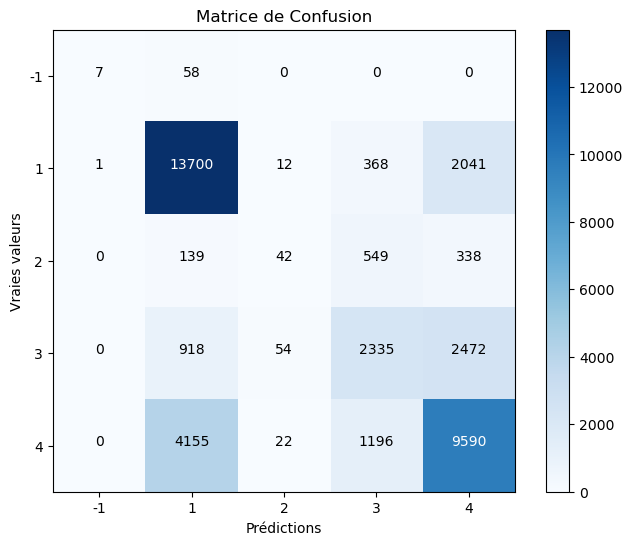
\includegraphics[width=0.8\textwidth]{img/confusionmatrix.png}
  \caption{Resultat de la classification produite par le RandomTreeClassifier : Gravité en variable cible.
  (-1 : Non renseigné
  1 : Indemne
  2 : Tué
   3: Blessé hospitalisé
   4 : Blessé léger)}
  \label{fig:nom_figure}
\end{figure}

\begin{table}[h]
  \centering
  \begin{tabular}{|c|c|c|c|c|}
    \hline
    \textbf{Gravité} & \textbf{Précision} & \textbf{Rappel} & \textbf{F1-Score} & \textbf{Support} \\
    \hline
    \textbf{Non renseigné} & 0.88 & 0.11 & 0.19 & 65 \\
    \hline
    \textbf{Indemne} & 0.72    &  0.85   &   0.78   &  16122 \\
    \hline
    \textbf{Tué} & 0.32   &   0.04   &   0.07   &   1068 \\
    \hline
    \textbf{Blessé hospitalisé} & 0.52   &   0.40   &   0.46   &   5779 \\
    \hline
    \textbf{Blessé léger} & 0.66   &   0.64   &   0.65  &   14963 \\
    \hline
  \end{tabular}
  \caption{Évaluation des performances du modèle. Variable cible : Gravité}
  \label{tab:evaluation_modele}
\end{table}

Nous pouvons voir que le modèle choisi n'est pas exactement égal pour tout les cas.
\begin{itemize}

    \item Non renseigné: Bien que la précision soit élevée (0,88), le rappel est très faible (0,11), indiquant des difficultés du modèle à identifier correctement cette classe. Cela pourrait être dû à un manque d’exemples d’entraînement, comme le suggère le faible support (65).

    \item Indemne: Le modèle semble bien performer pour cette classe, avec une précision de 0,72 et un rappel de 0,85.

    \item Tué: Le modèle rencontre des difficultés à classer correctement cette classe, avec une précision et un rappel faibles (0,32 et 0,04 respectivement). Cela pourrait être dû à un manque d’exemples d’entraînement, comme le suggère le support relativement faible (1068).

    \item Blessé hospitalisé: Le modèle montre une performance modérée pour cette classe, avec une précision de 0,52 et un rappel de 0,40.

    \item Blessé léger: Le modèle affiche une performance décente pour cette classe, avec une précision de 0,66 et un rappel de 0,64.
\end{itemize}



\begin{figure}[h]
  \centering
  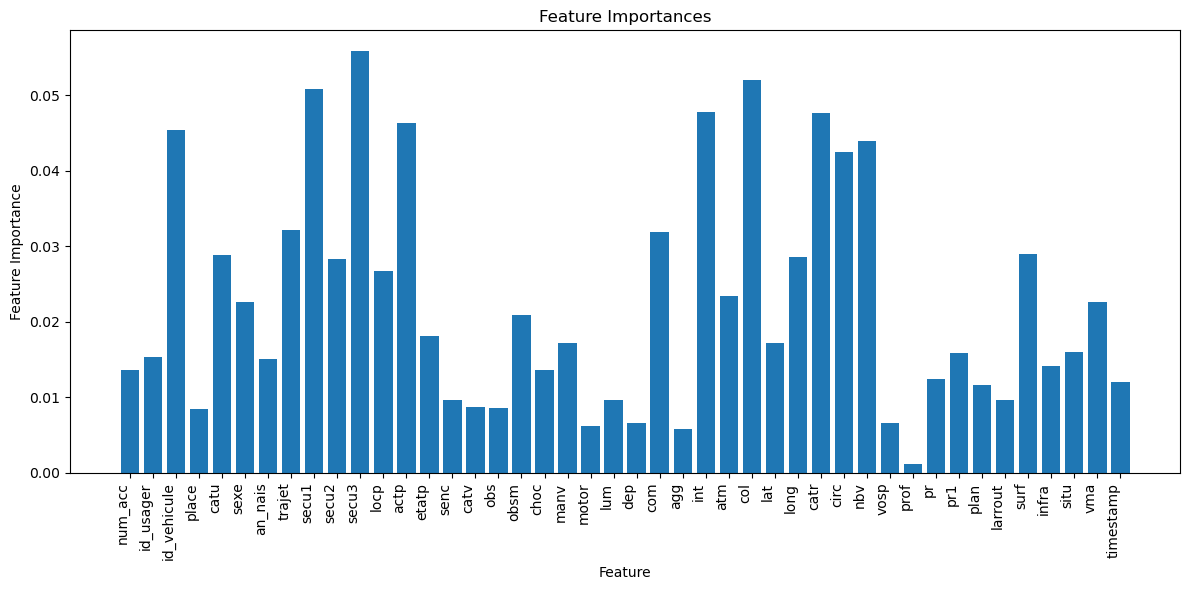
\includegraphics[width=0.8\textwidth]{img/feature_importance.png}
  \caption{Pertinence des variables dans la prediction de la gravité de l'accident}
  \label{fig:nom_figure}
\end{figure}

Sur le graphique illustrant l'importance des caractéristiques, nous constatons que les caractéristiques les plus pertinentes sont celles liées aux équipements de sécurité \verb|secu1| et \verb|secu3| utilisés dans chaque accident. Ces caractéristiques s'avèrent également pertinentes pour déterminer le type de blessure résultant de l'accident(\verb|col|).

Ces informations peuvent être complétées par l'action du piéton(\verb|actp|), qui fournit des indications précieuses sur les circonstances de l'accident. De plus, l'identifiant du véhicule (\verb|id_vehicule|) offre un aperçu intéressant des types de véhicules les plus susceptibles de causer des blessures lors d'un accident.

En somme, ces caractéristiques jouent un rôle crucial dans la prédiction de la gravité  des accidents de la route et peuvent nous aider à développer des stratégies plus efficaces pour prévenir ces accidents et minimiser leurs conséquences.

\section{Conclusion}
La classification des accidents de la route en France à l'aide de cet algorithme révèle les facteurs les plus importants à prendre en compte pour limiter les victimes.


La présence d'équipement de sécurité semble être le facteur le plus déterminant. La sensibilisation sur la nécessité de ces équipements est crucial et pourrait contribuer sans doute à réduire le nombre de blessés.


Le type de route et la localisation de l'accident semblent également jouer grandement sur la gravité des accidents. Il est donc important d'identifier ces lieux problématiques et de prendre les mesures nécessaires.


Enfin, dans les transports en commun, il est à souligner que certaines places offrent une meilleur sécurité en cas d'accident.


\newpage


\addcontentsline{toc}{section}{Bibliographie}
\bibliographystyle{unsrt}
\bibliography{sample}

\newpage

\appendix

\section{Choix des caractéristiques}

\begin{table}[!ht]
    \centering
    \begin{tabular}{|l|l|}
    \hline
        Name & Description \\ \hline
        num\_acc & Identifiant de l’accident \\ \hline
        id\_usager & Identifiant unique de l’usager \\ \hline
        id\_vehicule & Identifiant unique du véhicule repris pour chacun des usagers occupant ce véhicule \\ \hline
        place & Permet de situer la place occupée dans le véhicule par l'usager au moment de l'accident \\ \hline
        catu & Catégorie d'usager \\ \hline
        grav & Gravité de blessure de l'usager \\ \hline
        sexe & ~ \\ \hline
        an\_nais & Année de naissance de l’usager \\ \hline
        trajet & Motif du déplacement au moment de l’accident \\ \hline
        secu1 - secu2 - secu3 & Présence et utilisation d’un équipement de sécurité \\ \hline
        locp & localisation du piéton (0 si sans objet) \\ \hline
        actp & Action du piéton \\ \hline
        etatp & Cette variable permet de préciser si le piéton accidenté était seul ou non \\ \hline
        senc & Sens de circulation \\ \hline
        catv & catégorie du véhicule \\ \hline
        obs & Obstacle fixe heurté \\ \hline
        obsm & Obstacle mobile heurté \\ \hline
        choc & Point de choc initial \\ \hline
        manv & Manoeuvre principale avant l’accident \\ \hline
        motor & Type de motorisation du véhicule \\ \hline
        lum & Conditions d’éclairage \\ \hline
        dep & Code du département \\ \hlinehttps://www.overleaf.com/project/65607c210d395f473a6af25a
        agg & Localisation (Hors agglo ou en agglo) \\ \hline
        int & intersection \\ \hline
        atm & Conditions atmosphériques \\ \hline
        col & Type de collision \\ \hline
        lat & Latitude \\ \hline
        long & Longitude \\ \hline
        catr & Catégorie de route \\ \hline
        circ & Régime de circulation \\ \hline
        nbv & Nombe total de voies de circulation \\ \hline
        vosp & Signale l’existence d’une voie réservée \\ \hline
        prof & "Profil en long, décrit la déclivité de la route à l’endroit de l’accident" \\ \hline
        pr & Numéro de la borne amont \\ \hline
        pr1 & Distance par rapport à la borne amont \\ \hline
        plan & Tracé en plan \\ \hline
        larrout & "Largeur de la chaussée hors bande d’arrêt d’urgence, TPC et stationnement" \\ \hline
        surf & Etat de la surface \\ \hline
        infra & Aménagement \\ \hline
        situ & Situation \\ \hline
        vma & Vitesse maximale autorisée sur le lieu et au moment de l’accident \\ \hline
        timestamp & Heure de l’accident \\ \hline
    \end{tabular}
\end{table}




\end{document}